\chapter{Zadanie 5.}
Wyniki symulacji, podczas kt�rej nast�puje skokowa zmiana sygna�u zak��cenia wida� na rysunku ~\ref{dmc_skok_zakl}. Zmiana nast�pi�a w momencie ustabilizowania si� uk�adu po skoku warto�ci sterowania. Na wykresach wida�, �e algorytm, uwzgl�dniaj�cy zak��cenia (linia przerywana) radzi sobie lepiej, ni� klasyczny dmc, gdy� powr�t do warto�ci zadanej nast�puje du�o szybciej. Parametr $D^{z}$, tj. chwila, w kt�rej uk�ad stabilizuje si� po skoku warto�ci zak��cenia wynosi ok. $ 80 $, jednak w zale�no�ci od parametru $ \lambda $ mo�e by� du�o ni�szy.

\begin{figure}[b]
\centering
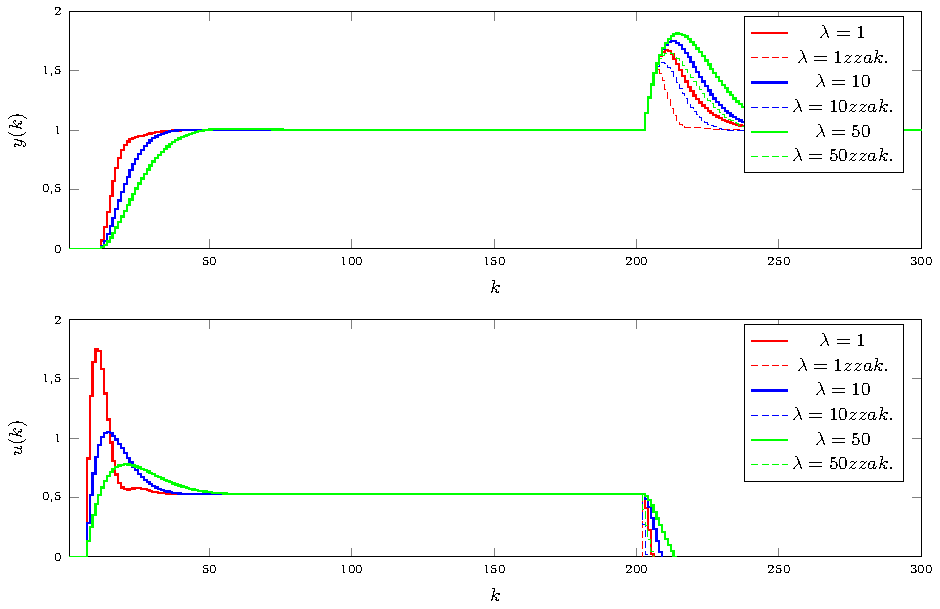
\includegraphics[scale=1]{../wykresy_pdf/zad5_dmc_zbiorczy.pdf}
\caption {Symulacja algorytmu DMC dla skoku zak��cenia}
\label{dmc_skok_zakl}
\end{figure}